\documentclass[12pt, a4paper]{article}

\usepackage{lastpage}
\usepackage{mathtools}
\usepackage{xltxtra}
\usepackage{libertine}
\usepackage{amsmath}
\usepackage{amsthm}
\usepackage{amsfonts}
\usepackage{amssymb}
\usepackage{enumitem}
\usepackage{xcolor}
\usepackage[left=1.5cm, right=1.5cm, top=2cm, bottom=2cm, bindingoffset=0cm, headheight=15pt]{geometry}
\usepackage{fancyhdr}
\usepackage[russian]{babel}
% \usepackage[utf8]{inputenc}
\usepackage{catchfilebetweentags}
\usepackage{accents}
\usepackage{calc}
\usepackage{etoolbox}
\usepackage{mathrsfs}
\usepackage{wrapfig}

\providetoggle{useproofs}
\settoggle{useproofs}{false}

\pagestyle{fancy}
\lfoot{M3137y2019}
\rhead{\thepage\ из \pageref{LastPage}}

\newcommand{\R}{\mathbb{R}}
\newcommand{\Q}{\mathbb{Q}}
\newcommand{\C}{\mathbb{C}}
\newcommand{\Z}{\mathbb{Z}}
\newcommand{\B}{\mathbb{B}}
\newcommand{\N}{\mathbb{N}}

\newcommand{\const}{\text{const}}

\newcommand{\teormin}{\textcolor{red}{!}\ }

\DeclareMathOperator*{\xor}{\oplus}
\DeclareMathOperator*{\equ}{\sim}
\DeclareMathOperator{\Ln}{\text{Ln}}
\DeclareMathOperator{\sign}{\text{sign}}
\DeclareMathOperator{\Sym}{\text{Sym}}
\DeclareMathOperator{\Asym}{\text{Asym}}
% \DeclareMathOperator{\sh}{\text{sh}}
% \DeclareMathOperator{\tg}{\text{tg}}
% \DeclareMathOperator{\arctg}{\text{arctg}}
% \DeclareMathOperator{\ch}{\text{ch}}

\DeclarePairedDelimiter{\ceil}{\lceil}{\rceil}
\DeclarePairedDelimiter{\abs}{\left\lvert}{\right\rvert}

\setmainfont{Linux Libertine}

\theoremstyle{plain}
\newtheorem{axiom}{Аксиома}
\newtheorem{lemma}{Лемма}

\theoremstyle{remark}
\newtheorem*{remark}{Примечание}
\newtheorem*{exercise}{Упражнение}
\newtheorem*{consequence}{Следствие}
\newtheorem*{example}{Пример}
\newtheorem*{observation}{Наблюдение}

\theoremstyle{definition}
\newtheorem{theorem}{Теорема}
\newtheorem*{definition}{Определение}
\newtheorem*{obozn}{Обозначение}

\setlength{\parindent}{0pt}

\newcommand{\dbltilde}[1]{\accentset{\approx}{#1}}
\newcommand{\intt}{\int\!}

% magical thing that fixes paragraphs
\makeatletter
\patchcmd{\CatchFBT@Fin@l}{\endlinechar\m@ne}{}
  {}{\typeout{Unsuccessful patch!}}
\makeatother

\newcommand{\get}[2]{
    \ExecuteMetaData[#1]{#2}
}

\newcommand{\getproof}[2]{
    \iftoggle{useproofs}{\ExecuteMetaData[#1]{#2proof}}{}
}

\newcommand{\getwithproof}[2]{
    \get{#1}{#2}
    \getproof{#1}{#2}
}

\newcommand{\import}[3]{
    \subsection{#1}
    \getwithproof{#2}{#3}
}

\newcommand{\given}[1]{
    Дано выше. (\ref{#1}, стр. \pageref{#1})
}

\renewcommand{\ker}{\text{Ker }}
\newcommand{\im}{\text{Im }}
\newcommand{\grad}{\text{grad}}

\lhead{Дифференциальные уравнения}
\cfoot{}
\rfoot{1.9.2020}

\setcounter{section}{-1}

\begin{document}

\section{Введение}

Пусть мы хотим найти $y$ --- функцию от одного аргумента.

\begin{definition}
    $F(x, y, y', \ldots, y^{(n)}) = 0$ --- \textbf{дифференциальное уравнение}
\end{definition}

\begin{example}
    Условие задачи:
    $$d y_n \approx k y_n d t$$
    $$\frac{d y}{d t} \approx ky$$
    \begin{equation}
        y' = ky
    \end{equation}
    $$y(t) = ?$$
    Предположим, что $y=kt$ --- решение искомого дифференциального уравнения. Подставим $y=kt$ в (1).
    $$(kt)' = k (kt)$$
    $$k = k^2t$$
    $$1 = kt$$
    $$t = \frac{1}{k}$$
    Это не верно для всех $t$, следовательно $y=kt$ --- не решение.

    Предположим, что $y=e^{kt}$ --- решение.
    $$(e^{kt})' = ke^{kt}$$
    $$ke^{kt} = ke^{kt}$$
    $$e^{kt} = e^{kt}$$
    Это верно $\forall t \in (-\infty, +\infty)$.

    Кроме того, $y=Ce^{kt}$ --- решение $\forall C\in\R$
\end{example}

\begin{example}
    Груз массой $m$ подвешен к пружине. Пусть его положение --- функция $x(t)$.

    В положении равновесия:
    $$mg = -kx_0$$

    Второй закон Ньютона:
    $$F_\Sigma = ma$$
    $$mg + (-k(x-x_0))= m \ddot x$$
    \begin{remark}
        $\ddot x \defeq \frac{d^2 x}{d t^2}$ \textit{(вторая производная $x$ по $t$)}
    \end{remark}
    $$-kx_0 - kx + kx_0 = m\ddot x$$
    $$-kx = m\ddot x$$
    Это дифференциальное уравнение второго порядка.

    Ответ: $$x(t) = A \sin\left(t\sqrt{\frac{k}{m}} + \phi_0\right)$$
    $A, \phi_0$ --- произвольные постоянные.
\end{example}

% Заметим, что в первом примере уравнение было первого порядка и в ответе была одна постоянная, а во втором примере уравнение было второго порядка, в ответе было две постоянных.

\section{Уравнения первого порядка. Основные понятия.}

\subsection{Уравнение первого порядка и его решения}

\begin{definition}
    $F(x, y, y')=0$ --- \textbf{уравнение первого порядка}
\end{definition}

\begin{definition}
    \textbf{Решением} уравнения первого порядка на $(a,b)$ называется функция $\varphi \in C^1(a,b)$:
    $$F(x, \varphi(x), \varphi'(x)) \equiv 0 \quad \forall x\in(a,b)$$

    ($a$ и $b$ могут быть $\infty$)
\end{definition}

\begin{example}
    $$\sphericalangle y'=x$$
    $$y = \frac{x^2}{2} + C$$
    $$\text{Частные решения: } \begin{cases}
            \varphi(x) = \frac{x^2}{2} \text{ --- решение на } (-\infty, +\infty) \\
            \varphi(x) = \frac{x^2}{2} + 1
        \end{cases}$$
\end{example}

\begin{definition}
    \textbf{Общее решение} --- множество всех решений.
\end{definition}

\begin{definition}
    \textbf{Общий интеграл} --- соотношение вида $F(x, y, C) = 0$, которое при любом допустимом $C$ неявно задаёт решение.
\end{definition}

\begin{example}
    $$y - \frac{x}{2} + C = 0 \text{ --- общий интеграл}$$
\end{example}

\begin{definition}
    \textbf{Интегральная кривая} уравнения --- график его решения.
\end{definition}

\subsection{Формы записи уравнения первого порядка}

\begin{definition}
    $y'=f(x,y)$ --- уравнение, \textbf{разерешенное относительно производной} \textit{(нормальная форма)}.
\end{definition}

\begin{example}
    $$\sphericalangle y' = -\frac{x}{y}$$
    $$y = \sqrt{1 - x} \text{ --- решение на } x\in(-1, 1)$$
    $$y = -\sqrt{1 - x} \text{ --- решение на } x\in(-1, 1)$$
    Кроме того, можно решить относительно $x$:
    $$\frac{dx}{dy} = -\frac{y}{x}$$
    $$x = \sqrt{1 - y} \text{ --- решение на } y\in(-1, 1)$$
    $$x = -\sqrt{1 - y} \text{ --- решение на } y\in(-1, 1)$$
\end{example}

\begin{definition}
    $P(x, y)dx + Q(x, y)dy = 0$ --- \textbf{уравнение в дифференциалах}
\end{definition}

\begin{definition}
    \textbf{Решением уравнения в дифференциалах} называется функция $y(x)\in C^1(a,b)$, такая что:
    $$P(x, y(x)) + Q(x, y(x)) y'(x) \equiv 0 \quad \forall x\in(a,b)$$
\end{definition}

Аналогично определяется решение $x(y)$.

\begin{definition}
    \textbf{Параметрическим решением уравнения в дифференциалах} называется пара $\varphi, \psi \in C^1(\alpha, \beta)$, такая что:
    \begin{enumerate}
        \item $|\varphi'(t)| + |\psi'(t)| > 0$
        \item $P(\varphi(t), \psi(t))\varphi'(t) + Q(\varphi(t), \psi(t))\psi'(t) \equiv 0 \quad \forall t\in (\alpha, \beta)$
    \end{enumerate}
\end{definition}

\begin{remark}
    Первое условие гарантирует, что в графике нет изломов, т.к. мы всегда ``движемся'' хотя бы по одной из осей.
\end{remark}

\begin{definition}
    \textbf{Интегральная кривая уравнения в дифференциалах} --- кривая, параметризация которой является параметрическим решением.
\end{definition}

\begin{example}
    $$ydy + xdx = 0$$

    Параметрическое решение: $\begin{cases}
            x(t) = \cos t \\
            y(t) = \sin t
        \end{cases}$
\end{example}

\subsection{Поле направлений и приближенные решения}

$\sphericalangle y'=f(x, y)$

$G$ --- область в $\R^2$

$f\in C(G)$

Пусть $\varphi$ --- решение на $(a, b)$, т.е. $\varphi'(x) = f(x, \varphi(x)) \quad \forall x\in(a,b)$

$y_0 := \varphi(x_0)$

$\varphi'(x_0) = f(x_0, y_0)$

$(1, f(x_0, y_0))$ --- касательный вектор к $y(x)$ в точке $x_0$

Построив множество касательных векторов, можно увидеть, как должны идти искомые кривые, т.к. они должны касаться этих векторов.

\begin{figure}[h]
    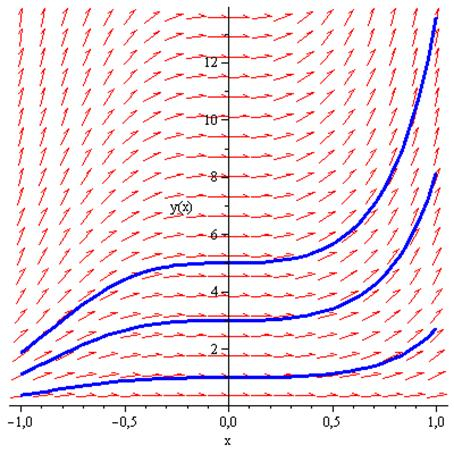
\includegraphics[scale=0.7]{images/dirfield.jpg}
    \centering
    \caption{Поле направлений с ломаными Эйлера}
\end{figure}

\begin{definition}[Ломаная Эйлера]
    $\sphericalangle y'=f(x, y), (x_0, y_0)$ --- начальная точка, $\Delta x$ --- постоянный шаг.

    Вершины \textbf{ломаной Эйлера}: $\begin{cases}
            x_k = x_0 + k\Delta x \\
            y_k = y_{k-1} + f(x_{k-1}, y_{k-1})\Delta x
        \end{cases}$
\end{definition}

\subsection{Задача Коши}

\begin{definition}
    \textbf{Задача Коши} \textit{(начальная задача)} для уравнения $y'=f(x, y)$ --- задача отыскать его решения, удовлетворяющие начальному условию $y(x_0)=y_0$, где $x_0, y_0$ --- начальные данные задачи.
\end{definition}

\begin{example}
    $$y'=2x \quad y(1)=2$$
    Решение:
    $$y=x^2+C$$
    $$y(1)=2 \Rightarrow 2 = 1 + C \Rightarrow C = 1$$
    Ответ: $y=x^2+1, x\in(-\infty, +\infty)$
\end{example}

\end{document}